
\section{Preliminary  Comparisons}
\label{Sec:Comparison}
\subsection{Performance profiles}
\frame{
  \frametitle{Performance profiles~\cite{Dolan.More2002}}

  \begin{itemize}
  \item Given a set of problems $\mathcal P$
  \item Given a set of solvers $\mathcal S$  
  \item A performance measure for each problem  with a solver $t_{p,s}$ (cpu time, flops, ...)
  \item Compute the performance ratio
    \begin{equation}
      \label{eq:perf-ratio}
      \tau_{p,s} =    \Frac{t_{p,s}}{\min_{s\in\mathcal S} t_{p,s}} \geq 1
    \end{equation}
  \item Compute the performance profile $\rho_s(\tau) : [1,+\infty]\rightarrow [0,1]$ for each solver $s\in \mathcal S$
    
    \begin{equation}
      \rho_s(\tau) = \Frac{1}{|\mathcal P|}\big|\{p\in \mathcal P\mid \tau_{p,s} \leq \tau    \}\big|\label{eq:perf}
  \end{equation}
  The value of $\rho_s(1)$ is the probability that the solver $s$ will win over the rest of the solvers.
  \end{itemize}
  
  
}
\begin{frame}
  \frametitle{LMGC90 sheared low wall example}
  \begin{figure}[htbp]
  \centering
  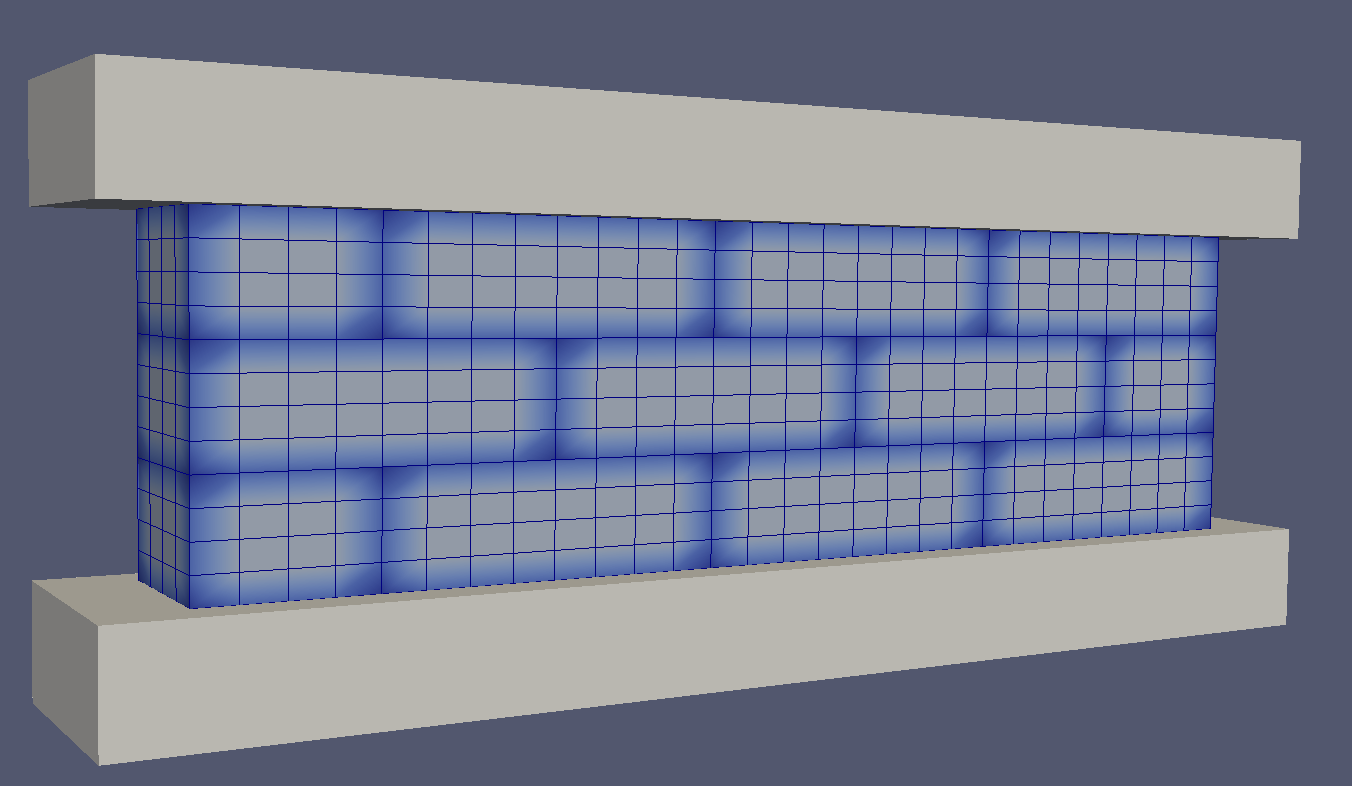
\includegraphics[height=0.5\textheight]{../figure/LowWall_FEM.png}
  \caption{A low wall meshes with H8}
  \label{fig:LowWall_FEM}
\end{figure}
\vspace{-0.5cm}
\begin{itemize}
\item H8 FE with Linear elastic behavior :
  $\rho= \num{2000}\si{\kilogram\per\cubic\metre},
  E=\num{2.2e+9}\si{\pascal} ,\nu = 0.2$
\item $\mu= 0.83 $ between block and $\mu =0.53$ between blocks and supports
\item Vertical compression force : $30000 \si{\newton}$ horizontal shear velocity $\num{1e-3}\si{\meter\per\second}$.
\item Sampling of $50$ problems collected in the FCLib with graded difficulty 
\end{itemize}
\end{frame}



\begin{frame}
  \frametitle{Results}
  \begin{figure}[htbp]
    \begin{center}
  \centering 
  \subfloat[Accuracy $\epsilon = 10^{-2}$]{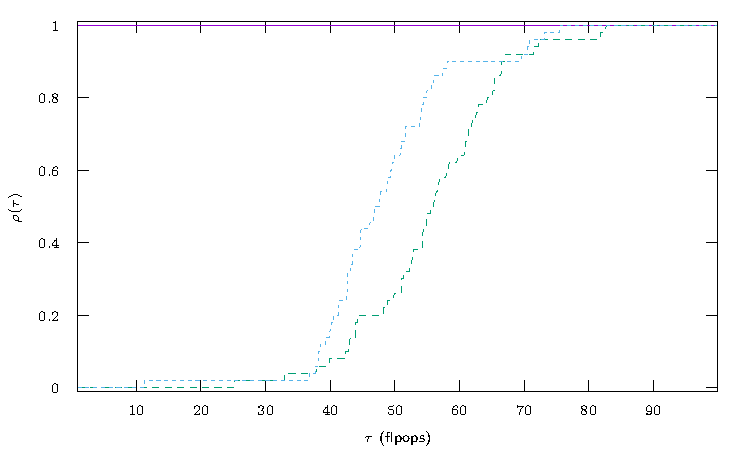
\includegraphics[width=0.55\textwidth]{../figure/LowWall_FEM.1e-2.with_guess/simple/profile-LMGC_LowWall_FEM.pdf}\label{fig:LowWall_FEM.1e-2.simple}}
   \subfloat[Accuracy $\epsilon = 10^{-3}$]{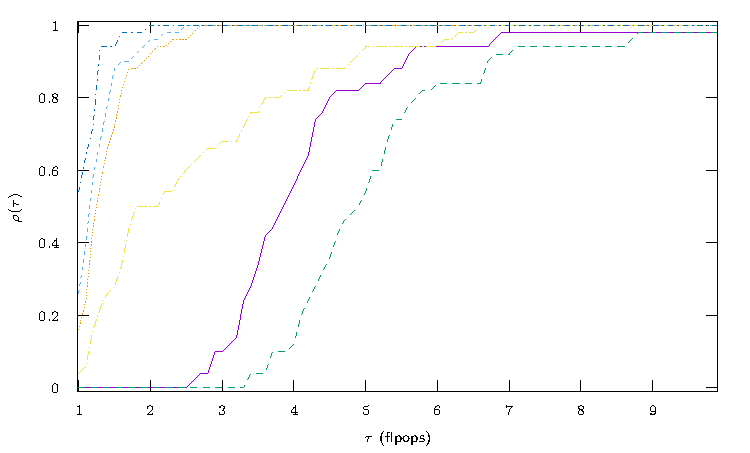
\includegraphics[width=0.55\textwidth]{../figure/LowWall_FEM.1e-3.with_guess/simple/profile-LMGC_LowWall_FEM.pdf}\label{fig:LowWall_FEM.1e-3.simple}}\\
   %\subfloat[Accuracy $\epsilon =  10^{-4}$]{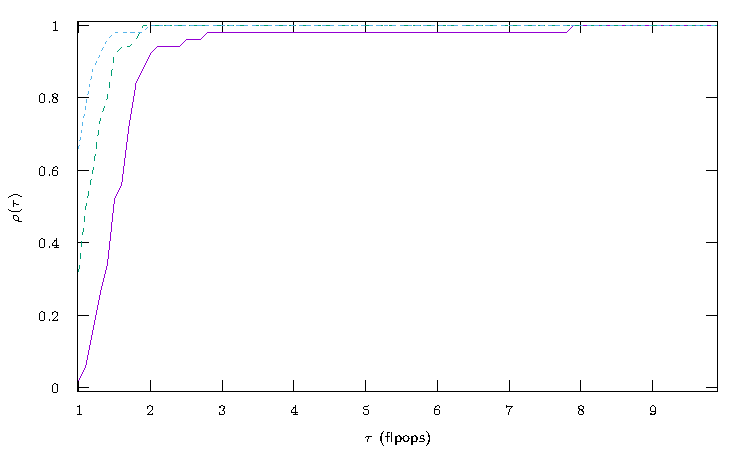
\includegraphics[width=0.49\textwidth]{../figure/LowWall_FEM.1e-4.with_guess/simple/profile-LMGC_LowWall_FEM.pdf}\label{fig:LowWall_FEM.1e-4.simple}}
   %\subfloat[Accuracy $\epsilon = 10^{-6}$]{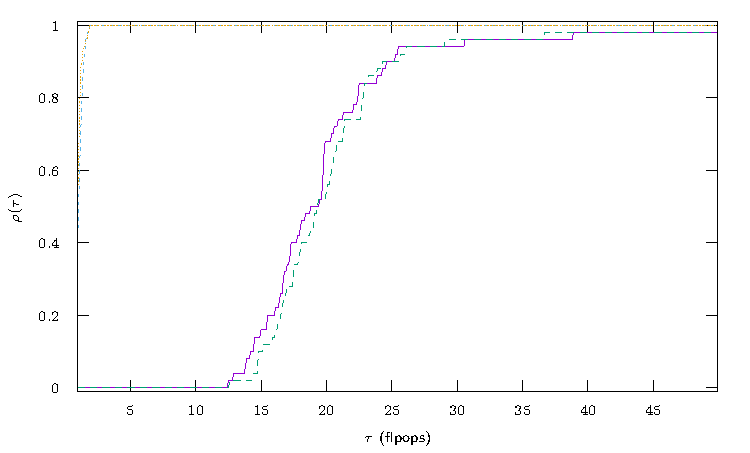
\includegraphics[width=0.49\textwidth]{../figure/LowWall_FEM.1e-6.with_guess/simple/profile-LMGC_LowWall_FEM.pdf}\label{fig:LowWall_FEM.1e-6.simple}}\\
   % \subfloat[précision $\epsilon = 10^{-8}$]{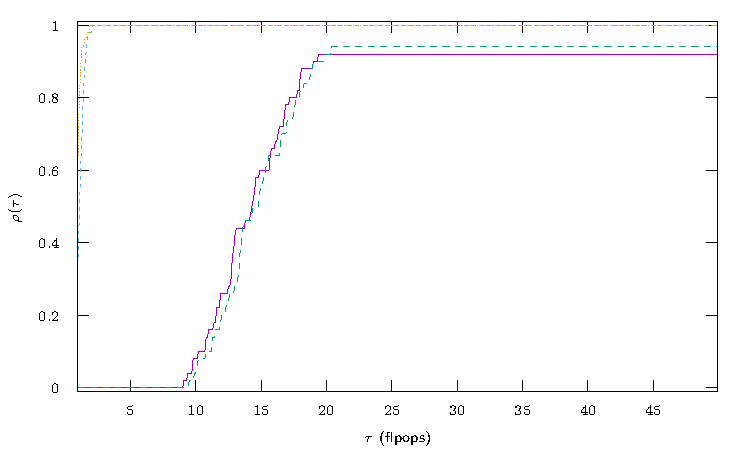
\includegraphics[width=0.49\textwidth]{figure/LowWall_FEM.1e-8.with_guess/simple/profile-LMGC_LowWall_FEM.pdf}\label{fig:LowWall_FEM.1e-8.simple}}\\
   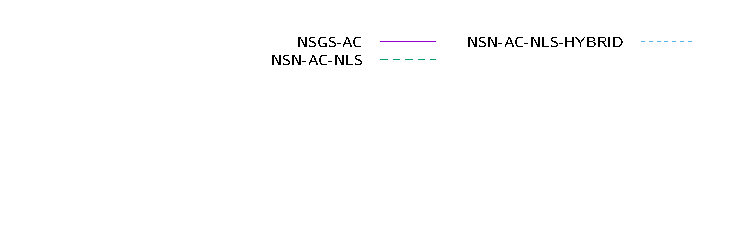
\includegraphics{../figure/LowWall_FEM.1e-2.with_guess/simple/profile-LMGC_LowWall_FEM_legend.pdf}
 \end{center}
  \caption{Comparison for two different required accuracies}
  \label{fig:LowWall_FEM.simple}
\end{figure}
\end{frame}

\begin{frame}
  \frametitle{Results}
  \begin{figure}[htbp]
  \centering 
  %\subfloat[Accuracy $\epsilon = 10^{-2}$]{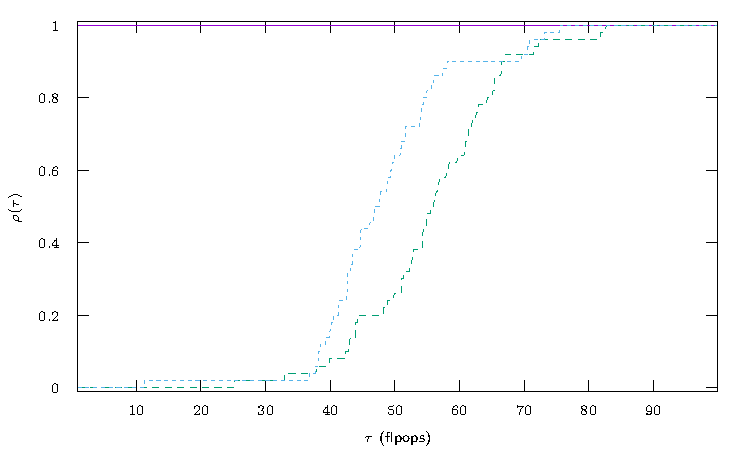
\includegraphics[width=0.49\textwidth]{../figure/LowWall_FEM.1e-2.with_guess/simple/profile-LMGC_LowWall_FEM.pdf}\label{fig:LowWall_FEM.1e-2.simple}}
  % \subfloat[Accuracy $\epsilon = 10^{-3}$]{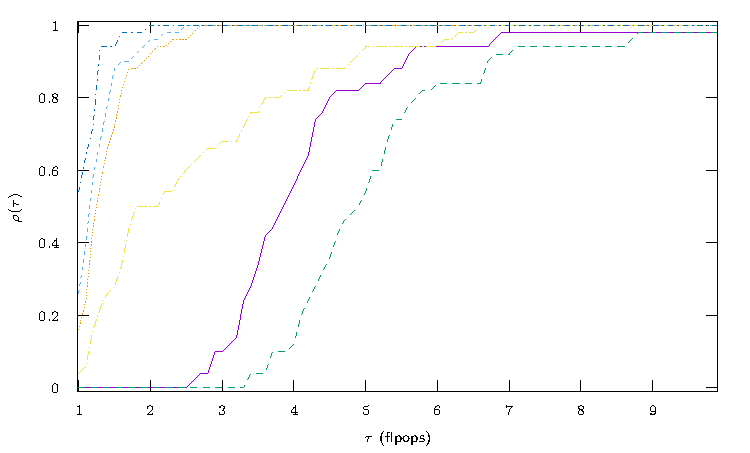
\includegraphics[width=0.49\textwidth]{../figure/LowWall_FEM.1e-3.with_guess/simple/profile-LMGC_LowWall_FEM.pdf}\label{fig:LowWall_FEM.1e-3.simple}}\\
   \subfloat[Accuracy $\epsilon =  10^{-4}$]{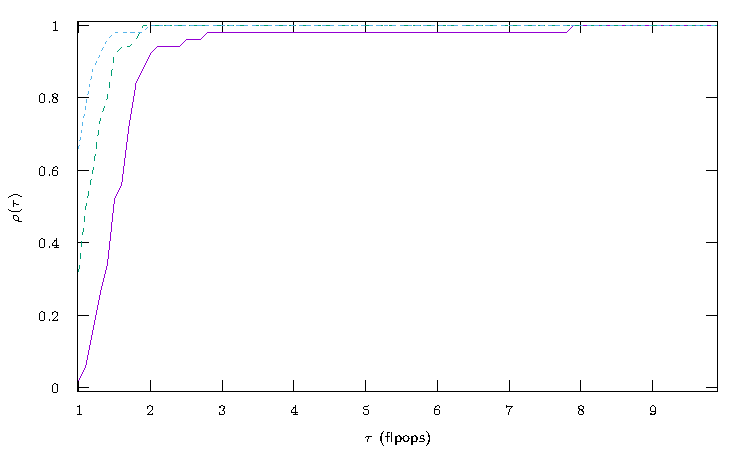
\includegraphics[width=0.55\textwidth]{../figure/LowWall_FEM.1e-4.with_guess/simple/profile-LMGC_LowWall_FEM.pdf}\label{fig:LowWall_FEM.1e-4.simple}}
   \subfloat[Accuracy $\epsilon = 10^{-6}$]{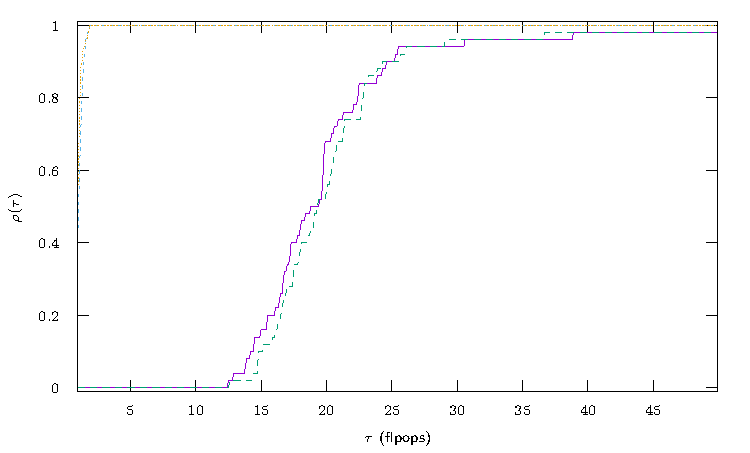
\includegraphics[width=0.55\textwidth]{../figure/LowWall_FEM.1e-6.with_guess/simple/profile-LMGC_LowWall_FEM.pdf}\label{fig:LowWall_FEM.1e-6.simple}}\\
   % \subfloat[précision $\epsilon = 10^{-8}$]{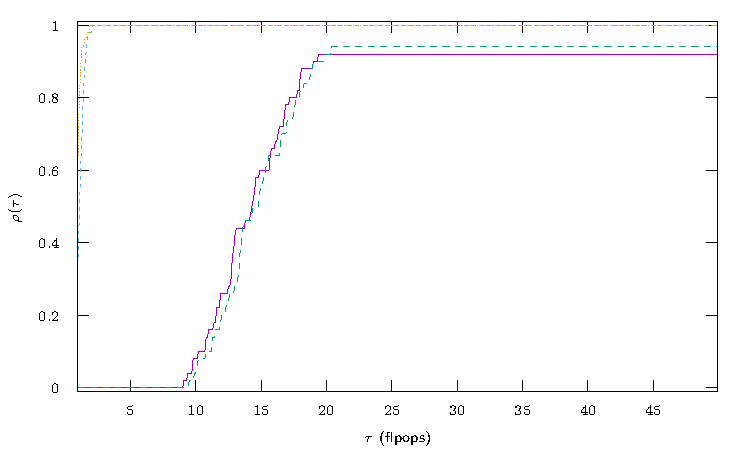
\includegraphics[width=0.49\textwidth]{figure/LowWall_FEM.1e-8.with_guess/simple/profile-LMGC_LowWall_FEM.pdf}\label{fig:LowWall_FEM.1e-8.simple}}\\
   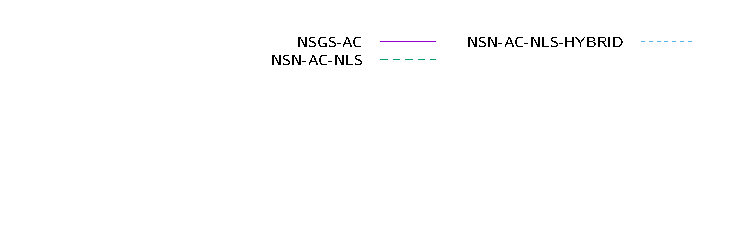
\includegraphics{../figure/LowWall_FEM.1e-2.with_guess/simple/profile-LMGC_LowWall_FEM_legend.pdf}
  \caption{Comparison for two different required accuracies}
  \label{fig:LowWall_FEM.simple}
\end{figure}
\end{frame}
%%% Local Variables:
%%% mode: latex
%%% TeX-master: "s"
%%% End:

